\subsection*{Partie I. La fonction.}
\begin{enumerate}
  \item Les conditions se traduisent par un système de 3 équations aux inconnues $a$, $b$, $c$
\begin{displaymath}
  \left\lbrace  
  \begin{aligned}
    a - b + c &= 0 \\  c &= 1\\  a + b + c &= -1
  \end{aligned}
\right. 
\Leftrightarrow
  \left\lbrace  
  \begin{aligned}
    c &= 1\\ a - b &= -1 \\ a + b &= -2
  \end{aligned}
\right. 
\Leftrightarrow
  \left\lbrace  
  \begin{aligned}
    c &= 1\\ a &= -\frac{3}{2} \\ b &= -\frac{1}{2}
  \end{aligned}
\right. 
\end{displaymath}
La seule fonction polynomiale $f$ de degré $2$ vérifiant $f(-1)=0$, $f(0)=1$ et $f(1)=-1$ est donc
\begin{displaymath}
  f(x) = -\frac{3}{2}x^2 - \frac{1}{2}x + 1
\end{displaymath}

  \item Le graphe présenté est bien celui d'une fonction du second degré (parabole) dont le coefficient de $x^2$ est strictement négatif. Le calcul de la dérivée permet d'obtenir $m$ et $b=f(m)$.
\begin{displaymath}
  f'(x) = -3x - \frac{1}{2} \hspace{0.5cm}\Rightarrow \hspace{0.5cm} m = -\frac{1}{6} \hspace{0.5cm}\text{ et }\hspace{0.5cm} b = \frac{25}{24}
\end{displaymath}
La recherche des points fixes se fait en résolvant $f(x) -x=0$
\begin{multline*}
  f(x) -x = -\frac{3}{2}x^2 - \frac{3}{2}x + 1, \hspace{0.5cm} 
  \Delta = \frac{33}{4}\Rightarrow\\
  a = -\frac{\sqrt{33} + 3}{6}\simeq -1.46, \hspace{0.5cm} a' = \frac{\sqrt{33} - 3}{6}\simeq 0.46
\end{multline*}
Sur le graphe figurent aussi les trois points fondamentaux
\begin{displaymath}
(-1,0)=(-1,f(-1)),\hspace{0.5cm} (0,1)=(0,f(0)),\hspace{0.5cm}(1,-1)=(1,f(1))
\end{displaymath}

  \item La fonction $f$ est strictement croissante sur $\left] -\infty , a\right]$ et diverge vers $-\infty$ en $-\infty$ donc
\begin{displaymath}
  f\left( \left]  -\infty , a\right]\right) = \left]  -\infty , f(a)\right] = \left] -\infty , a\right] \text{ car $a$ est un point fixe.}
\end{displaymath}
La fonction est strictement croissante aussi sur $\left[ a, m \right]$ donc 
\begin{displaymath}
  f\left( \left[ a, m \right]\right) = \left[ f(a) , f(m) \right] = \left[ a, b \right] \; \text{ car } b = f(m).
\end{displaymath}
La fonction est strictement décroissante sur $\left[ m, b \right]$ donc 
\begin{displaymath}
  f\left( \left[ m, b \right]\right) = \left[ f(b) , f(m) \right] = \left[ f(b), b \right]\subset \left[ a,b\right] \hspace{1cm}\left( \text{ car } a < f(b)\right) 
\end{displaymath}
Comme $f\left( \left[ a, m \right]\right)$ et $f\left( \left[ m, b \right]\right)$ sont inclus dans $\left[ a,b\right]$, le segment $\left[ a,b\right]$ est stable.  
  \item L'intervalle $\left] -\infty , a\right]$ est stable donc la suite définie par récurrence par la condition initiale $x_0$ avec $x_0<a$ est bien définie et tous les $x_n$ sont dans $\left] -\infty , a\right]$. De plus $f(x_0)<x_0$ d'après l'étude des signes et la fonction $f$ est strictement croissante dans l'intervalle considéré. On en tire
\begin{displaymath}
  x_1 < x_0 \Rightarrow x_2 = f(x_1) < f(x_0) = x_1 \Rightarrow \cdots 
\end{displaymath}
La suite est donc décroissante et tous les $x_n$ sont strictement plus petits que $x_0$ donc plus petits que $a$. Si la suite convergeait, comme $f$ est continue, sa limite serait un point fixe de $f$ strictement plus petit que $a$. Or il n'existe pas de tel point fixe donc la suite diverge vers $-\infty$.\newline
Si $x_0=a$ ou $a'$ (points fixes), la suite est constante de valeur $a$ ou $a'$.\newline
Si $x_0=-1$ ou $0$ ou $1$, la suite est périodique de période $3$. Elle prend successivement les valeurs $-1$, $0$, $1$.
\end{enumerate}

\subsection*{Partie II. Les outils.}
\begin{enumerate}
  \item On suppose $[u,v]\subset g([u,v])$. Comme l'énoncé nous y invite, considérons $z$ et $t$ dans $[u,v]$ tels que $g(z)=u$ et $g(t)=v$. Considérons aussi la fonction (évidemment continue)
\begin{displaymath}
  \varphi: \;
  \left\lbrace 
  \begin{aligned}
    \left[ u,v\right] &\rightarrow \R \\
    x &\mapsto g(x) - x
  \end{aligned}
\right. 
\end{displaymath}
Alors:
\begin{align*}
\varphi(z) = g(z) -z = u-z \leq 0 &\text{ car } z\in \left[ u,v\right] \\
\varphi(t) = g(t) -t = v-t \geq 0 &\text{ car } t\in \left[ u,v\right]
\end{align*}
Si une des inégalités est une égalité, elle est associée à un point fixe. Si les deux inégalités sont strictes, on peut appliquer le théorème des valeurs intermédiaires dans l'intervalle d'extrémités $z$ et $t$. Il existe $c$ entre $z$ et $t$ tel que $\varphi(c)=0$ c'est à dire $g(c) = c$.
  \item Comme $[v,V] \subset f(I)$, il existe $a$ et $b$ dans $I$ tels que $f(a)=v$ et $f(b)=V$. On suppose dans les trois premières sous-questions que $a<b$.
\begin{enumerate}
  \item La partie $A$ est non vide car elle contient $a$. Comme elle est par définition incluse dans $[a,b]$, elle est majorée par $b$. Elle admet donc (propriété fondamentale de $\R$) une borne supérieure notée $\alpha$. De $a\in A$, on déduit $a\leq \alpha$ et de $b$ majorant de $A$, on déduit $\alpha \leq b$ donc $\alpha \in [a,b]$.\newline
  D'après le cours, $\alpha$ est la limite d'une suite $\left( a_n\right)_{n\in \N}$ d'éléments de $A$ qui converge vers $\alpha$. La suite $\left( f(a_n)\right)_{n\in \N}$ est constante de valeur $v$ (par définition de $A$) et elle converge vers $f(\alpha)$ car $f$ est continue en $\alpha$. On obtient donc $f(\alpha)=v$ c'est à dire $\alpha\in A$ donc $\alpha = \max A$.\newline
  Comme $\alpha = \max A$, si $x \in \left]\alpha ,b\right]$ alors $x\notin A$ donc $f(x) \neq v$.\newline
  Si $f(x)< v$, on applique le théorème des valeurs intermédiaires dans $\left[x,b\right]$ et il existe $c\in \left] x,b\right[$ tel que $f(c)=v$ en contradiction avec $\alpha = \max A$. Ceci montre que $f(x)>v$.     
  \item On raisonne comme dans la question précédente. La partie $B$ est non vide (car $b \in B$), minorée par $\alpha$ (car $B\subset [\alpha, b]$); elle admet donc une borne inférieure $\beta\in [\alpha,b]$. On approche $\beta$ par une suite d'éléments de $B$, on en déduit $f(\beta)=V$ par continuité de $f$ en $\beta$ donc $\beta\in B$ et $\beta=\min B$.\newline
  Comme $\beta = \min B$, si $x \in \left[\alpha ,\beta\right[$ alors $x\notin B$ donc $f(x) \neq V$.\newline
  Si $f(x)> V$, on applique le théorème des valeurs intermédiaires dans $\left[\alpha, x\right]$ et il existe $c\in \left]\alpha, x\right[$ tel que $f(c)=V$ en contradiction avec $\beta = \min B$. Ceci montre que $f(x) < V$.     
  
  \item Les implications des questions a. et b. montrent que $f([\alpha,\beta])\subset [v,V]$. Réciproquement, pour tout $y\in ]v,V[ = ]f(\alpha),f(\beta)[$, il existe $x \in]\alpha, \beta[$ tel que $f(x)=y$ à cause du théorème des valeurs intermédiaires.
  \item Dans le cas où $b < a$, on peut se ramener au cas traité en considérant la fonction $x\mapsto f(-x)$ qui a pour effet de renverser le domaine de définition.
\end{enumerate}

\end{enumerate}

\begin{figure}[h]
  \centering
  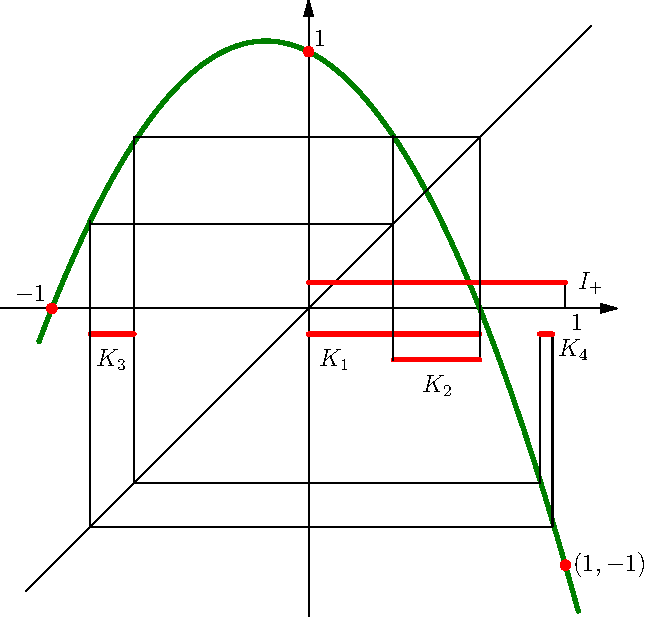
\includegraphics{./Cp3impko_1.pdf}
  % Ep3impko_1.pdf: 0x0 pixel, -2147483648dpi, 0.00x0.00 cm, bb=
  \caption{Segments $K_1$, $K_2$, $K_3$, $K_4$}
  \label{fig: Cp3impko_1}
\end{figure}

\subsection*{Partie III. Existence de suites périodiques.}
\begin{enumerate}
  \item D'après l'étude des variations de la première partie 
\begin{displaymath}
f(I_-) = [0,f(m)] = [0,b]  
\end{displaymath}
Comme $1 < b$, on a bien $I_+=[0,1]\subset [0,b]=f(I_-)$.\newline
Dans $I_+$ la fonction est décroissante
\begin{displaymath}
  f(I_+) = f([0,1]) = [f(1),f(0)] = [-1,1] = I_- \cup I_+
\end{displaymath}
On en déduit $I_- \subset f(I_+)$ et $I_+ \subset f(I_+)$.

  \item
\begin{enumerate}
  \item Comme $I_+ \subset f(I_+)$, le résultat de la question II.2. montre qu'il existe un segment $K_1\subset I_+$ tel que $f(K_1) = I_+$.\newline
  De même $K_1 \subset I_+$ s'écrit aussi $K_1 \subset f(K_1)$ par définition de $K_1$. On peut encore appliquer II.2.: il existe $K_2 \subset K_1\subset I_+$ tel que $f(K_2) = K_1$.\newline
  Utilisons maintenant $I_+ \subset f(I_-)$, on en déduit $K_2\subset f(I_-)$ car $K_2\subset I_+$. Toujours d'après II.2., il existe $K_3\subset I_-$ tel que $f(K_3)=K_2$.\newline
  Utilisons enfin $I_-\subset f(I_+)$. De $K_3\subset I_- \subset f(I_+)$, on déduit avec II.2. qu'il existe $K_4\subset I_+$ tel que $f(K_4) = K_3$. 
  \item La segments estimés graphiquement sont présentés en figure \ref{fig: Cp3impko_1}. Ils sont légèrement décalés verticalement de l'axe des abscisses pour être mieux visibles.
\end{enumerate}

  \item Par construction des segments $f(K_1)=I_+$, $f(K_2)=K_1$, $f(K_3)=K_2$ et $f(K_4)=K_3$. On en déduit $f^4(K_4) = I_+$ donc 
\begin{displaymath}
  K_4 \subset f^4(K_4)
\end{displaymath}
car $K_4 \subset I_+$. On peut appliquer la question II.1. avec la fonction continue $g=f^4$. Il existe donc un $c\in K_4$ tel que $f^4(c) = c$.
  
  \item D'après la définition des segments:  
\begin{multline*}
  \left( c\in K_4 \Rightarrow c\in I_+\right), \hspace{0.5cm} 
  \left( f(c)\in f(K_4)=K_3 \Rightarrow f(c)\in I_-\right), \hspace{0.5cm}\\
  \left( f^2(c)\in f(K_3)=K_2 \Rightarrow f^2(c)\in I_+\right), \\
  \left( f^3(c)\in f(K_2)=K_1 \Rightarrow f^3(c)\in I_+\right)
\end{multline*}
Si $c=f(c)$ alors ce nombre est dans $I_+\cap I_-$ donc $c=0$ ce qui est impossible car $f(0)=1$.\newline
Si $c=f^2(c)$ alors $f(c)=f^3(c)$ donc ce nombre est dans $I_+\cap I_-$ donc $f(c)=0$ ce qui est impossible car $f^3(c)=f^2(0)=-1$.\newline
De même $c=f^3(c)$ est impossible car cela entraine $f(c)=f^4(c)=c$ déjà traité. On en conclut que $c$ répond bien à la question. La suite définie par  récurrence à partir de $c$ est périodique de plus petite période $4$.
  
  \item Comme $I_+ \subset f(I_-)$, d'après II.2., il existe $J_1\subset I_-$ tel que $f(J_1)=I_+$. Comme $I_-\subset f(I_+)$, il existe $J_2\subset I_+$ tel que $f(J_2)=J_1$. On a donc $f^2(J_2)= I_+$ puis $J_2 \subset f^2(J_2)$. On peut appliquer II.1. à $f^2$ et en déduire l'existence d'un point fixe $c_2\in J_2\subset I_+$ de $f^2$. Comme $f(c_2)\in J_1 \subset I_-$, $f(c_2)=c_2$ impliquerait $c_2=0$ ce qui est absurde. 
  
  \item On peut supposer $n\geq 5$ car les cas $n=2$ et $4$ ont été traités et $0$ est de période $3$ par définition. On utilise la même méthode que pour 4 et reprenant les mêmes notations.
\begin{multline*}
I_+\subset f(I_+) \Rightarrow \exists K_1\subset I_+ \text{ tq } f(K_1)=I_+ \\ 
K_1 \subset I_+ = f(K_1) \Rightarrow \exists K_2\subset K_1 \text{ tq } f(K_2) = K_1 \\
K_2 \subset K_1 = f(K_2) \Rightarrow \exists K_3\subset K_2 \text{ tq } f(K_3) = K_2 \\
\cdots \\
K_{n-3} \subset K_{n-4} = f(K_{n-3}) \Rightarrow \exists K_{n-2}\subset K_{n-3} \text{ tq } f(K_{n-2}) = K_{n-3} \\
K_{n-2} \subset I_+ = f(I_-) \Rightarrow \exists K_{n-1}\subset I_- \text{ tq } f(K_{n-1}) = K_{n-2} \\
K_{n-1} \subset I_- = f(I_+) \Rightarrow \exists K_{n}\subset I_+ \text{ tq } f(K_{n}) = K_{n-1} 
\end{multline*}
On a fabriqué ainsi un segment $K_n\subset I_+$ tel que $f^n(K_n)=I_+$ donc $K_n \subset f^n(K_n)$ donc (II.1. appliqué à $f^n$ dans $K_n$) il existe $c_n\in K_n$ tel que $f^n(c_n)=c_n$.\newline
Il reste à montrer que
\begin{displaymath}
  \forall k\in \llbracket 1,n-1\rrbracket, \; f^k(c_n)\neq c_n
\end{displaymath}
Remarquons que $c_n\in K_n \subset I_+$, $f(c_n)\in K_{n-1}\subset I_-$ et pour tous les $k\geq 2$, $f^k(c_n)\in I_+$. Autrement dit, tous les $f^k(c_n)$ sont dans $I_+$ sauf $f(c_n)$ qui est dans $I_-$ et on a déjà utilisé que l'intersection des deux intervalles se réduit à $0$.\newline
Si $f^{n-1}(c_n)=c_n$, en composant par $f$, on obtient $c_n = f(c_n)$ donc égal à $0$ ce qui est impossible.
Supposons $k\in \llbracket 1,n-2\rrbracket$ et $f^{k+1}(c_n)= f(c_n)$. On obtient une contradiction car l'un est dans $I_+$ et l'autre dans $I_-$. La plus petite période est donc bien $n$.
\begin{displaymath}
  c_n = f^n(c_n) = f^{n-k}(c_n)
\end{displaymath}

\end{enumerate}
